\documentclass[a4paper,10pt]{book}
\usepackage[utf8x]{inputenc}
% User defined settings
\usepackage{xspace}
\usepackage{psfrag}
\usepackage{todonotes}
\usepackage{xcolor}
\usepackage{natbib}
\usepackage{tabularx}
\usepackage{multicol}
\usepackage[verbose]{wrapfig}
\usepackage[colorlinks,bookmarks=true]{hyperref}
\usepackage{amsbsy,amsfonts,amsmath,amssymb,enumerate,epsfig,graphicx,rotating}
\usepackage[FIGTOPCAP,nooneline]{subfigure}

% \usepackage{mdframed}

%Mathematics
\newcommand{\f}[2]{\frac{#1}{#2}}
\newcommand{\dd}{\partial}
\newcommand{\de}{{\rm \, d}}
\newcommand{\mysec}[1]{{\noindent\bf #1.}}
\newcommand{\pn}{Prandtl number}
%-------- Vectors
\renewcommand{\vec}[1]{\mathbf{#1}}
\renewcommand{\v}{\vec}
\newcommand{\bec}{\vec}

%-------- Numbers
\newcommand{\Ra}{$Ra\ $}
\renewcommand{\P}{$P\ $}
\newcommand{\Nu}{$Nu\ $}
\renewcommand{\t}{$\tau\ $}
\newcommand{\Pm}{$P_m\ $}
\newcommand{\El}{$\Lambda\ $}
\newcommand\ie{i.e.\ }
\newcommand\etal{\mbox{\textit{et al.}}}
\newcommand\etc{etc.\ }
\newcommand\eg{e.g.\ }
\newcommand{\mypsfrag}[2]{\psfrag{#1}{\footnotesize{#2}}}
\newcommand{\warning}[1]{\vspace{1em}\fcolorbox{orange}{white}{\centering\parbox{0.9\textwidth}{{\Large\color{red} Warning}\vspace*{2mm}\newline#1}}\vspace{1em}}


\providecommand{\MD}{\textbf{MD}\xspace}
\providecommand{\FD}{\textbf{FD}\xspace}
\providecommand{\Mdip}{\ensuremath{{M}_\text{dip}}\xspace}
\providecommand{\Mmp}{\ensuremath{\overline{M}_p}\xspace}
\providecommand{\Mft}{\ensuremath{\widetilde{M}_t}\xspace}
\providecommand{\Mmt}{\ensuremath{\overline{M}_t}\xspace}
\providecommand{\Mfp}{\ensuremath{\widetilde{M}_p}\xspace}
\providecommand{\Emp}{\ensuremath{\overline{E}_p}\xspace}
\providecommand{\Efp}{\ensuremath{\widetilde{E}_p}\xspace}
\providecommand{\Emt}{\ensuremath{\overline{E}_t}\xspace}
\providecommand{\Eft}{\ensuremath{\widetilde{E}_t}\xspace}
\providecommand{\Ha}{\ensuremath{H_{\vec{_a}}}\xspace}
\providecommand{\Hu}{\ensuremath{H_{\vec{_u}}}\xspace}
\providecommand{\HB}{\ensuremath{H_{\vec{_B}}}\xspace}
\providecommand{\Hcross}{\ensuremath{H_\times}\xspace}
\providecommand{\MfpToMmp}{\ensuremath{\widetilde{M}_p/\overline{M}_p}\xspace}
\providecommand{\MfpToMmpD}{\ensuremath{\widetilde{M}_p^\mathrm{dip}/\overline{M
}_p^\mathrm{dip}}\xspace}

\allowdisplaybreaks
\usepackage{charter}

\title{DRS ($@DRS_VERSION@$) \\ A User's Manual}
\author{Luis Silva}

\begin{document}

\pagenumbering{alph}

\maketitle

\clearpage\pagenumbering{roman}

\tableofcontents

\clearpage\pagenumbering{arabic}
\chapter*{Introduction}
\addcontentsline{toc}{chapter}{Introduction}
This is the user manual for the DRS (\underline{D}ynamo in a
\underline{R}otating \underline{S}hell) code. API documentation can be found on
the online APIDOX.
Ported to f95 by Luis Silva (lacsilva@gmail.com)

\chapter{How to use this code}

\section{DEPENDENCIES}
We use \verb|cmake| version 2.8 as the build system.
We depend on \verb|FFTW3| version $>=$ 3.2.1. Tested up to version 3.3.3.
We use \verb|OpenMPI| $>=$ 1.6 for the parallel version. The binary wrappers must
be in your \verb|$PATH| and the libraries in your \verb|$LD_LIBRARY_PATH|.
Online documentation can be built using \verb|doxygen|  version $>=$ 1.6.1.
In order to compress the state files we use \verb|gzip|. Most unix systems will have it

\section{Compiling and installing the code}
The DRS code and utilities use the cmake build system in order to generate
native builds for *nix and Windows alike. Some features can be activated or
deactivated at compile time by passing the appropriate ``-D'' option to cmake.
Table~\ref{t:cmakeOptions} summarises the present set of feature options. Check
the cmake documentation \citep{CMakeDox} for other build options.

\begin{table}[htb]
\centering
 \begin{tabular}{lcp{0.6\textwidth}}
  Option & Values & Description\\ \hline
  & & \\
  MPI& ON/OFF& Activates/deactivates compilation of the parallel parts of the
code. OFF by default.\\
  COMP& ON/OFF& Activates/deactivates compilation of support for composition.
OFF by default.\\
  BUILD\_UTILS & ON/OFF & Activates/deactivates compilation of the utilities.
OFF by default.\\
  BUILD\_TESTS & ON/OFF & Activates/deactivates compilation of the unit tests.
OFF by default.\\
  BUILD\_DOCS  & ON/OFF & Build the user manual from the latex sources. ON by
default when pdflatex is found.
 \end{tabular}
\caption{List of options that activate/deactivate features at compile time.}
\label{t:cmakeOptions}
\end{table}

\subsection{Building the online documentation}
\begin{verbatim}
$ mkdir BUILD
$ cd BUILD
$ cmake ..
$ make doc
\end{verbatim}
The code documentation can then be found by pointing a browser
to:\\
\verb|<your favorite browser> BUILD/APIDOX/index.html|

\subsection{COMPILATION (sequential)}
\begin{verbatim}
$ mkdir BUILD
$ cd BUILD
$ cmake ..
$ make && make install
\end{verbatim}
After all run successfully, the file drs.exe should be in \verb|bin/|.

\subsection{COMPILATION (parallel)}
\begin{verbatim}
$ mkdir BUILD
$ cd BUILD
$ cmake -DMPI=ON ..
$ make && make install
\end{verbatim}
After all run successfully, the file drs.exe should be in the \verb|bin/|
folder of the source code folder.

\section{Running DRS}
\subsection{Command-line options}
Since version 1.6.1, DRS acceps the \verb|-v| command line option.
When this option is used the program will write the version and compile time
options and exit with code 1.

\subsection{Before running DRS}
\label{s:runConfig}
Each run needs to be configured. Configuration is passed on the standard input
and obeys a format similar to the following.
\begin{small}
\begin{verbatim}
[Filenames]
io_calc_file_in = state_in
io_calc_file_out = state_out

# Parameters describing the geometry.
[Geometry]
# Aspect ratio
eta = 0.35
# Equatorial symmetry
lsymm = 0
# Azimuthal symmetry
m0 = 1
# Radial resolution
Nr = 33
# Meridional resolution
Nt = 64
# Azimuthal resolution
Np = 129
# Spectral resolutions
Nr_s = 33
Nt_s = 64
Np_s = 129

# Parameters describing the boundary conditions.
# Check drsDefs.f90.in for the definitions.
[Boundaries]
# Purely conductive profile
tempProf = 0
# Fixed temperature at the boundaries
tempBC_i = 0
tempBC_o = 0
# No slip boundary conditions
flowBC_i = 1
flowBC_o = 1
# Insulating boundaries
magBC_i = 0
magBC_o = 0

# adimensional parameters to be used.

[Adimensional]
# Taylor
Ta = 4.0d6
# Thermal Prandtl
Pt = 1.0d0
# Magnetic Prandtl
Pm = 5.0d0
# Rayleigh thermal
Ra_t = 1.0d5

# Parameters that controll the runtime aspects of the simulation.
[Runtime]
# Input/output data format.
lform = 0
# Calculation to be performed.
drs_calc_type = 4
# Simulation time step.
h = -1.0d-6
# Maximum number of time steps.
stepmax = 20000
# Maximum cpu time in hours
cpu_max_time = 2
# Should we sample on simulation time (true/T/.T. or false/F/.F.)
sample_on_sim_time=.F.
# How many steps constitute a transient.
transient = 0
# Sampling rate in terms of the number of steps.
sample_rate = 100
# Intermediate state save rate in terms of the number of steps.
state_save_rate = 500
# Should we have a save rate in simulation time
state_save_on_sim_time=.F.
# A comment describing the calculation.
comment = A comment describing the calculation.
# Some noise in the initial temperature.
noise = 0.0d0
\end{verbatim}
\end{small}

Possible values for the computation type, \verb|drs_calc_type|, are:
\begin{itemize}
\item[1] \verb|LinearThermalOnset|
\item[2] \verb|KinematicDynamo|
\item[3] \verb|NonlinearConvection|
\item[4] \verb|NonlinearDynamo|
\item[5] \verb|MagnetoConvection|
\item[6] \verb|LinearCompositionalOnset|
\end{itemize}
Add 10 to include composition.

Possible values for the boundary conditions are 0 or 1 according to the following
table:
\begin{table}[htb]
\begin{tabular}{c|l|l|l|l}
Opt. & \verb|temBC|      & \verb|compBC|       & \verb|flowBC| & \verb|magBC|  \\ \hline
0     & Fixed temperature & Fixed composition   & Free slip     & Vacuum        \\
1     & Fixed heat flux   & Fixed chemical flux & No slip       & Pseudo-vacuum \\
\end{tabular}
\caption{Possible values for the the boundary conditions and their meanings.}
\end{table}

In the folder where DRS is run, the program must also be able to find the
initial state files. These contain the coefficients for the flow, temperature,
magnetic field, etc. A typical directory listing prior to the execution looks
like:
\begin{small}
\begin{verbatim}
 > ll
total 680K
-rw------- 1 user group 130K Sep 30 15:56 e035p1t2r100000m1p5.1.Bp.gz
-rw------- 1 user group 129K Sep 30 15:56 e035p1t2r100000m1p5.1.Bt.gz
-rw------- 1 user group  528 Nov 12 12:34 e035p1t2r100000m1p5.1.par
-rw------- 1 user group 131K Sep 30 15:56 e035p1t2r100000m1p5.1.pol.gz
-rw------- 1 user group 129K Sep 30 15:56 e035p1t2r100000m1p5.1.temp.gz
-rw------- 1 user group 129K Sep 30 15:56 e035p1t2r100000m1p5.1.temp.BC
-rw------- 1 user group 129K Sep 30 15:56 e035p1t2r100000m1p5.1.tor.gz
-rwx--x--x 1 user group 4.2K Nov 20 15:42 jobscript-parallel
-rwx--x--x 1 user group 4.3K Nov 26 12:27 jobscript-serial
\end{verbatim}
\end{small}

Notice that the input state files are compressed using unix gzip. This is
due to space saving requirements. Decompression of these files is dealt
with by the \verb|jobscrit-*| scripts described below. The file with extension
\verb|.par| describes the structure and contents of the other files. \verb|.par|
files are described in section~\ref{s:parFiles}. Extensions
\verb|.pol| and \verb|.tor| are for the coefficients of the poloidal and
toroidal flow. Similarly, \verb|.Bp| and \verb|.Bt| are for the coefficients of
the poloidal and toroidal magnetic field. Extension \verb|.temp| refers to the
temperature. See section~\ref{s:inputs} for details on the structure of the
\verb|.par| and state files.

\subsection{Running on one CPU}
\subsection{Running on multiple CPU's with MPI}

\section{A variety of queueing systems}
Because some preparation is needed prior to running DRS and because some
post-processing (like storing the output data in a predetermined place) may be
needed, we recommend using job scripts. Typically, these scripts will be
adapted to run under a queueing system that provides resource and I/O
management and may require modifications to the pre/post processing. A few
examples of these job scripts follow for a variety of queueing systems.

\warning{Note that execution is usually timed and and the queue will mercilessly kill
your job once the walltime is reached. Make sure you set a walltime for drs that is
smaller than the queue walltime so that setup tasks, main program and cleanup
tasks can be executed. You may lose your data if you don't!}

\subsection{No queueing system}

\begin{small}
\begin{verbatim}
#!/bin/bash
############################################################
######
######    Example shell script to serve as a job launcher
######    and controller.
######
#
#-------------------------------------------------
# Check the following settings before submitting!

# The base name of the state files before numbering.
file=MyJobFilename

# Where to find the utilities required to deal with the state files.
BINDIR=${HOME}/bin

# Where to find the program executale
command=${BINDIR}/drs.exe

# Number of the run on input
# This is overriden by the value in ${job}.num
numi=1

# Highest number of the run on output.
maxnum=10

# Construct the input/output file numbering.
numo=$((numi + 1))
infile="$file.$numi"
outfile="$file.$numo"

# The following few lines establish the parameters to be used in the
# computation. Create and check drs.conf.template carefully before
# running. The configuration template should have the
# @infile@ and @outfile@ placeholders in place of the required values.
sed -e "s/@infile@/$infile/g" \
    -e "s/@outfile@/$outfile/g" \
    drs.conf.template > ${job}.in

# Uncompress the input files
${BINDIR}/uncompressdata $infile

# Run the simulation
${command} < ${job}.in
\end{verbatim}
\end{small}

The format for \verb|drs.conf.template| is described in section
\ref{s:runConfig}. An occurrence of \verb|@infile@| and \verb|@outfile@| should
exist in that file so that they can be replaced by the appropriate values.


\subsection{SLURM}
The SLURM queueing system requires the above example to be slightly modified.
\begin{small}
\begin{verbatim}
#!/bin/bash
############################################################
######
######    Example shell script to serve as a job launcher
######    and controller.
######    This example is meant for execution of
######    the program the slurm queueing system.
######
#SBATCH -J myMPI        # Job name
#SBATCH -o myjob.%j.out # stdout output file (%j expands to jobId)
#SBATCH -e myjob.%j.err # stderr output file (%j expands to jobId)
#SBATCH -p development  # Queue name
#SBATCH -N 2            # Number of nodes requested (16 cores/node)
#SBATCH -n 32           # Number of mpi tasks requested
#SBATCH -t 12:00:00     # Run time (hh:mm:ss) - 1.5 hours
.
<setup tasks>
.
# Run the simulation
ibrun -n $NPROCS ${command} < ${job}.in
.
<cleanup tasks>
.
\end{verbatim}
\end{small}

\subsection{TORQUE/PBS}
The TORQUE/PBS style of queueing systems requires the above example to be
slightly modified.
\begin{small}
\begin{verbatim}
#!/bin/bash
############################################################
######
######    Example shell script to serve as a job launcher
######    and controller.
######    This example is meant for execution of
######    the program under the torque/pbs queueing system.
######
#PBS -N e07p075t20r180000m1p1-high-eb
#PBS -l nodes=1:ppn=4
#PBS -l walltime=48:00:00
#PBS -m bea -M luis.silva@glasgow.ac.uk
.
<setup tasks>
.
mpirun -np $NPROCS ${command} < ${job}i
.
<cleanup tasks>
.
\end{verbatim}
\end{small}

\chapter{Theory}

\section{Problem set up and approximations}
\label{s:problemSetup}
We consider a spherical fluid shell of inner radius $r_i$ and outer radius
$r_o$. The shell thickness is then $d = r_o - r_i$. The shell is rotating at
constant angular velocity $\Omega$ about an axis aligned with the $z$ direction.
Boundaries are impermeable and electrically insulating. Figure~\ref{f:setup}
shows a depiction of this geometry.
\begin{figure}[htb]
\centering
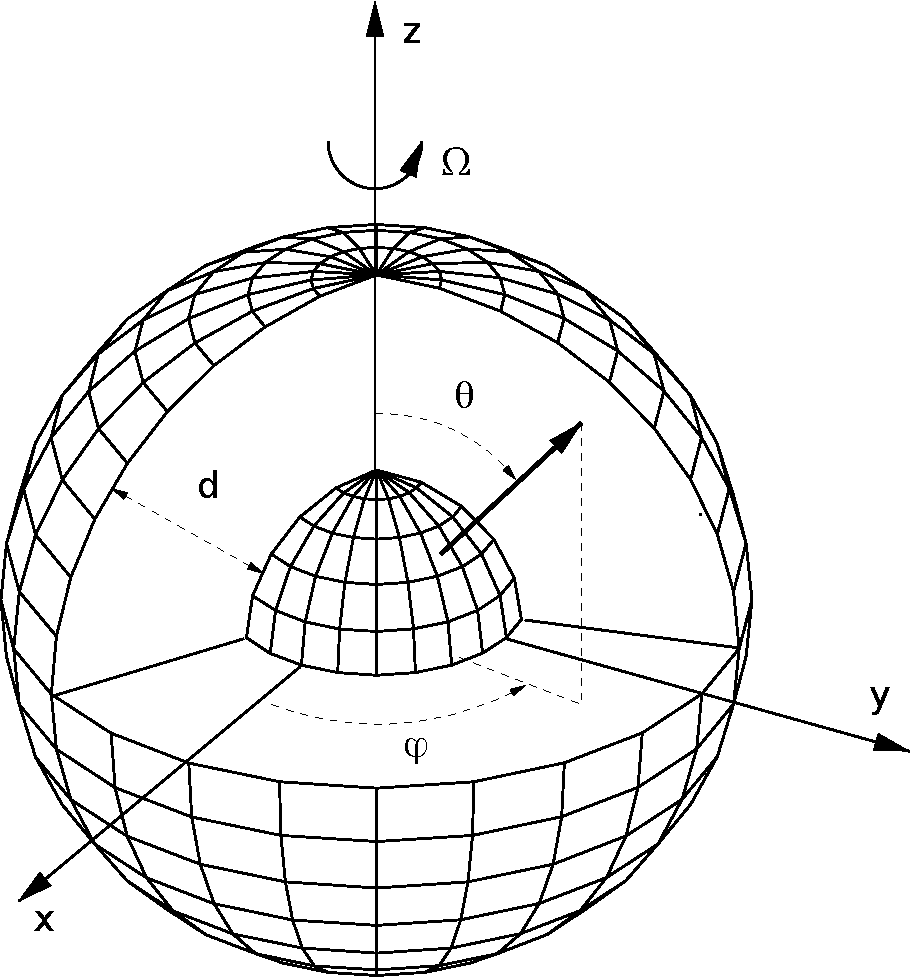
\includegraphics[width=0.5\textwidth]{figs/sphshell}
\caption{Depiction of the problem set-up.}
\label{f:setup}
\end{figure}

The fluid inside the shell is incompressible, electrically and thermally
conductive with magnetic diffusivity $\lambda$ and thermal diffusivity $\kappa$,
and has a viscosity $\nu$. Optionally, we can also consider that the fluid is a
nearly homogeneous mixture composed of a heavy solvent and a light solute with
chemical diffusivity $D$. The system is permeated by a magnetic field that
evolves in time through both advection and diffusion. The equations that
describe this system are then:
\begin{subequations}
\begin{gather}
\label{e:nonDivergenceDim}
\nabla \cdot \vec u = 0, \qquad \nabla \cdot \vec B = 0, \\
\label{e:NavierStokesDim}
\partial_t(\rho \vec u) = - \vec u \cdot \nabla (\vec u\rho) -
 2\rho\vec\Omega \times \vec u
 -\nabla P + \rho \vec{g} +
\vec\nabla\times(\nu\vec\nabla\times\vec{u})+ \vec{j}\times\vec B, \\
\label{e:temperatureDim}
\partial_t T = - \vec u \cdot \nabla T + \kappa \nabla^2 T + S_T, \\
\label{e:compositionDim}
\partial_t C = - \vec u \cdot \nabla C + \kappa \nabla^2 C + S_C, \\
\label{e:inductionDim}
\partial_t \vec B  =  - \vec u \cdot \nabla \vec B +  \vec B \cdot \nabla\vec u
+ \vec\nabla\times(\lambda\vec\nabla\times\vec{B}).
\end{gather}
\end{subequations}
An equation similar to \ref{e:temperatureDim} can be added that describes the
evolution of the concentration of the light solute. The system is closed with an
equation of state that describes the evolution of $\rho$ as a function of the
other variables.

Before we continue we are going to make a few more approximations. We will
assume that all diffusivities are constant both in time and space and that the
electric field is small enough and the electric conductivity is high enough that
there is no net charge imbalance. This last assumption leads to:
\begin{equation}
 \vec{j} = \frac{1}{\mu}\nabla\times\vec{B},
\end{equation}
with $\mu$ the magnetic permeability of the core material.

\subsection{The Boussinesq approximation}
Up until this point, the only approximations that were made relate to the fact
that the fluid is incompressible, that the electric field is deemed small on the
relevant time scales and all problem parameters are constant. Besides that, we
limited the body forces that act on the fluid to the viscous force and the
magnetic force. The flow is also heated in the volume by a non-descript source
$S$ which we will discuss later.

The Boussinesq approximation consists in making use of the yet unprescribed
equation of state to postulate that the density variations both in time and
space are negligeable except when it comes to their effect on the gravity term.
That is, $\rho = \rho_0$, except when it comes to the term $\rho \vec{g}$. There
we have:
\begin{equation}
 \rho \approx \rho_0 + \frac{\partial \rho}{\partial T}\delta T + \frac{\partial \rho}{\partial C}\delta C,
\label{e:thermodyn}
\end{equation}
where $C$ is the concentration of light solute. We can now identify the partial
derivatives with respect to the thermo-dynamic quantities as being related to
the thermal expansion factor and the compositional density reduction factor:
\begin{subequations}
\begin{gather}
\alpha_T = -\frac{1}{\rho_0}\frac{\partial \rho}{\partial T} \\
\alpha_C = -\frac{1}{\rho_0}\frac{\partial \rho}{\partial C}
\end{gather}
\label{e:factors}
\end{subequations}
Another consequence of the small density anomalies is that the gravity field,
$\vec{g}$, can be replaced by that of a sphere of uniform density, thus reducing
to:
\begin{equation}
 \vec{g} = -\gamma r \hat{r}
\label{e:grav}
\end{equation}
where $\gamma$ is a constant given in $s^{-2}$.

Replacing eq.~\ref{e:thermodyn}, \ref{e:factors} and \ref{e:grav} into
\ref{e:NavierStokesDim} we obtain:
\begin{equation}
\partial_t \vec u = - \vec u \cdot \nabla \vec u -
 2\vec\Omega \times \vec u -\nabla \Pi +  \gamma r \hat{r}(\alpha_T \delta T + \alpha_C \delta C) +
\frac{\nu}{\rho_0}\nabla^2\vec{u}+ \frac{1}{\mu\rho_0}(\vec\nabla\times\vec B )\times\vec B,
\end{equation}
where we introduced all the simplifications that we made so far and introduced
the generalized pressure gradient $-\nabla \Pi$. We will come back to the
Navier-Stokes equation in the next section.

The Boussinesq approximation has another more physically relevant consequence.
In order for one to be able to write eq.~\ref{e:thermodyn}, one must assume
that, at all times, both the temperature and the concentration must only
slightly depart from static (constant in time) underlying fields $T_S$ and
$C_S$. Furthermore, these fields must not be arbitrary, but reflect the average
state of the convection as buoyancy driven motion should only occur for
deviations from these states. It is usual to chose profiles that are spherically
symmetric and obey the temperature and composition
equations~\ref{e:temperatureDim} and~\ref{e:compositionDim} for a given set of
sources. Other choices, as is the case of a homogeneously distributed
concentration field are based upon observations.

In DRS we assume a static thermal state described by a radial temperature
profile $T_S (r)$ that can be one of the values described in
Table~\ref{t:t_profiles}.
\begin{table}[htb]
\centering
\begin{tabular}{|c|lp{0.48\textwidth}|}\hline
 Opt. & Equation & Description\\\hline
  &                          & \\
 0&$T_S(r) = T_0 + \beta(r_i r_o/r - r_i)$ & The conductive temperature
 profile used in \citep{ChristensenEtAl01}. See Section~\ref{bench:Christ01}.
 \\\hline
  &                          & \\
 1&$T_S(r) = T_0 - \beta r^2/2$    & This profile closely
follows the adiabat \citep{LabrossePoirier1997,DaviesGubbins2011} and alludes to
the possibility that at least a fraction of the energy available to planetary
dynamos is due to radiogenic heat release. \\ \hline
\end{tabular}
\caption{Possible temperature profiles, in K, hardcoded into DRS. First column
refers to the option values used in the code.}
\label{t:t_profiles}
\end{table}
Note that the conductive profile exactly obeis eq.~\ref{e:temperature} with
$S_T=0$ and that the quasi-adiabatic profile emulates a non-zero volumetric
heat source.

Constants $T_0$ and $\beta$ have values that depend on the profile and can be
written, in dimensional form, as a function of the temperature at the top
($T_o$) and bottom ($T_i$) boundaries. Opt.~0 has $T_0 = T_o$ and $\beta = (T_i
-T_o)/d$ and refers to the same temperature profile used in the first dynamo
benchmark exercise \citep{ChristensenEtAl01} whereas Opt.~1 has $T_0 = (T_i
r_o^2 - T_o r_i^2)/(r_o^2 - r_i^2)$ and $\beta = (T_o - T_i)/(r_o^2 - r_i^2)$,
thus closely following an adiabatic temperature profile
\citep{LabrossePoirier1997, DaviesGubbins2011}.
\begin{figure}[htb]
\centering % GNUPLOT: LaTeX picture
\setlength{\unitlength}{0.240900pt}
\ifx\plotpoint\undefined\newsavebox{\plotpoint}\fi
\begin{picture}(1500,900)(0,0)
\sbox{\plotpoint}{\rule[-0.200pt]{0.400pt}{0.400pt}}%
\put(191.0,131.0){\rule[-0.200pt]{300.643pt}{0.400pt}}
\put(191.0,131.0){\rule[-0.200pt]{4.818pt}{0.400pt}}
\put(171,131){\makebox(0,0)[r]{ 4000}}
\put(1419.0,131.0){\rule[-0.200pt]{4.818pt}{0.400pt}}
\put(191.0,222.0){\rule[-0.200pt]{300.643pt}{0.400pt}}
\put(191.0,222.0){\rule[-0.200pt]{4.818pt}{0.400pt}}
\put(171,222){\makebox(0,0)[r]{ 4200}}
\put(1419.0,222.0){\rule[-0.200pt]{4.818pt}{0.400pt}}
\put(191.0,313.0){\rule[-0.200pt]{300.643pt}{0.400pt}}
\put(191.0,313.0){\rule[-0.200pt]{4.818pt}{0.400pt}}
\put(171,313){\makebox(0,0)[r]{ 4400}}
\put(1419.0,313.0){\rule[-0.200pt]{4.818pt}{0.400pt}}
\put(191.0,404.0){\rule[-0.200pt]{300.643pt}{0.400pt}}
\put(191.0,404.0){\rule[-0.200pt]{4.818pt}{0.400pt}}
\put(171,404){\makebox(0,0)[r]{ 4600}}
\put(1419.0,404.0){\rule[-0.200pt]{4.818pt}{0.400pt}}
\put(191.0,495.0){\rule[-0.200pt]{300.643pt}{0.400pt}}
\put(191.0,495.0){\rule[-0.200pt]{4.818pt}{0.400pt}}
\put(171,495){\makebox(0,0)[r]{ 4800}}
\put(1419.0,495.0){\rule[-0.200pt]{4.818pt}{0.400pt}}
\put(191.0,586.0){\rule[-0.200pt]{300.643pt}{0.400pt}}
\put(191.0,586.0){\rule[-0.200pt]{4.818pt}{0.400pt}}
\put(171,586){\makebox(0,0)[r]{ 5000}}
\put(1419.0,586.0){\rule[-0.200pt]{4.818pt}{0.400pt}}
\put(191.0,677.0){\rule[-0.200pt]{300.643pt}{0.400pt}}
\put(191.0,677.0){\rule[-0.200pt]{4.818pt}{0.400pt}}
\put(171,677){\makebox(0,0)[r]{ 5200}}
\put(1419.0,677.0){\rule[-0.200pt]{4.818pt}{0.400pt}}
\put(191.0,768.0){\rule[-0.200pt]{213.919pt}{0.400pt}}
\put(1419.0,768.0){\rule[-0.200pt]{4.818pt}{0.400pt}}
\put(191.0,768.0){\rule[-0.200pt]{4.818pt}{0.400pt}}
\put(171,768){\makebox(0,0)[r]{ 5400}}
\put(1419.0,768.0){\rule[-0.200pt]{4.818pt}{0.400pt}}
\put(191.0,859.0){\rule[-0.200pt]{300.643pt}{0.400pt}}
\put(191.0,859.0){\rule[-0.200pt]{4.818pt}{0.400pt}}
\put(171,859){\makebox(0,0)[r]{ 5600}}
\put(1419.0,859.0){\rule[-0.200pt]{4.818pt}{0.400pt}}
\put(345.0,131.0){\rule[-0.200pt]{0.400pt}{175.375pt}}
\put(345.0,131.0){\rule[-0.200pt]{0.400pt}{4.818pt}}
\put(345,90){\makebox(0,0){ 1500}}
\put(345.0,839.0){\rule[-0.200pt]{0.400pt}{4.818pt}}
\put(621.0,131.0){\rule[-0.200pt]{0.400pt}{175.375pt}}
\put(621.0,131.0){\rule[-0.200pt]{0.400pt}{4.818pt}}
\put(621,90){\makebox(0,0){ 2000}}
\put(621.0,839.0){\rule[-0.200pt]{0.400pt}{4.818pt}}
\put(897.0,131.0){\rule[-0.200pt]{0.400pt}{175.375pt}}
\put(897.0,131.0){\rule[-0.200pt]{0.400pt}{4.818pt}}
\put(897,90){\makebox(0,0){ 2500}}
\put(897.0,839.0){\rule[-0.200pt]{0.400pt}{4.818pt}}
\put(1174.0,131.0){\rule[-0.200pt]{0.400pt}{150.803pt}}
\put(1174.0,839.0){\rule[-0.200pt]{0.400pt}{4.818pt}}
\put(1174.0,131.0){\rule[-0.200pt]{0.400pt}{4.818pt}}
\put(1174,90){\makebox(0,0){ 3000}}
\put(1174.0,839.0){\rule[-0.200pt]{0.400pt}{4.818pt}}
\put(191.0,131.0){\rule[-0.200pt]{0.400pt}{175.375pt}}
\put(191.0,131.0){\rule[-0.200pt]{300.643pt}{0.400pt}}
\put(1439.0,131.0){\rule[-0.200pt]{0.400pt}{175.375pt}}
\put(191.0,859.0){\rule[-0.200pt]{300.643pt}{0.400pt}}
\put(30,495){\rotatebox{-270}{\makebox(0,0){Temperature/K}}
}\put(815,29){\makebox(0,0){Radius/km}}
\put(1279,819){\makebox(0,0)[r]{Conduction}}
\put(1299.0,819.0){\rule[-0.200pt]{24.090pt}{0.400pt}}
\put(191,814){\usebox{\plotpoint}}
\multiput(191.58,811.16)(0.493,-0.734){23}{\rule{0.119pt}{0.685pt}}
\multiput(190.17,812.58)(13.000,-17.579){2}{\rule{0.400pt}{0.342pt}}
\multiput(204.58,792.09)(0.492,-0.755){21}{\rule{0.119pt}{0.700pt}}
\multiput(203.17,793.55)(12.000,-16.547){2}{\rule{0.400pt}{0.350pt}}
\multiput(216.58,774.29)(0.493,-0.695){23}{\rule{0.119pt}{0.654pt}}
\multiput(215.17,775.64)(13.000,-16.643){2}{\rule{0.400pt}{0.327pt}}
\multiput(229.58,756.23)(0.492,-0.712){21}{\rule{0.119pt}{0.667pt}}
\multiput(228.17,757.62)(12.000,-15.616){2}{\rule{0.400pt}{0.333pt}}
\multiput(241.58,739.54)(0.493,-0.616){23}{\rule{0.119pt}{0.592pt}}
\multiput(240.17,740.77)(13.000,-14.771){2}{\rule{0.400pt}{0.296pt}}
\multiput(254.58,723.54)(0.493,-0.616){23}{\rule{0.119pt}{0.592pt}}
\multiput(253.17,724.77)(13.000,-14.771){2}{\rule{0.400pt}{0.296pt}}
\multiput(267.58,707.51)(0.492,-0.625){21}{\rule{0.119pt}{0.600pt}}
\multiput(266.17,708.75)(12.000,-13.755){2}{\rule{0.400pt}{0.300pt}}
\multiput(279.58,692.67)(0.493,-0.576){23}{\rule{0.119pt}{0.562pt}}
\multiput(278.17,693.83)(13.000,-13.834){2}{\rule{0.400pt}{0.281pt}}
\multiput(292.58,677.65)(0.492,-0.582){21}{\rule{0.119pt}{0.567pt}}
\multiput(291.17,678.82)(12.000,-12.824){2}{\rule{0.400pt}{0.283pt}}
\multiput(304.58,663.80)(0.493,-0.536){23}{\rule{0.119pt}{0.531pt}}
\multiput(303.17,664.90)(13.000,-12.898){2}{\rule{0.400pt}{0.265pt}}
\multiput(317.00,650.92)(0.497,-0.493){23}{\rule{0.500pt}{0.119pt}}
\multiput(317.00,651.17)(11.962,-13.000){2}{\rule{0.250pt}{0.400pt}}
\multiput(330.58,636.79)(0.492,-0.539){21}{\rule{0.119pt}{0.533pt}}
\multiput(329.17,637.89)(12.000,-11.893){2}{\rule{0.400pt}{0.267pt}}
\multiput(342.00,624.92)(0.539,-0.492){21}{\rule{0.533pt}{0.119pt}}
\multiput(342.00,625.17)(11.893,-12.000){2}{\rule{0.267pt}{0.400pt}}
\multiput(355.58,611.79)(0.492,-0.539){21}{\rule{0.119pt}{0.533pt}}
\multiput(354.17,612.89)(12.000,-11.893){2}{\rule{0.400pt}{0.267pt}}
\multiput(367.00,599.92)(0.590,-0.492){19}{\rule{0.573pt}{0.118pt}}
\multiput(367.00,600.17)(11.811,-11.000){2}{\rule{0.286pt}{0.400pt}}
\multiput(380.00,588.92)(0.539,-0.492){21}{\rule{0.533pt}{0.119pt}}
\multiput(380.00,589.17)(11.893,-12.000){2}{\rule{0.267pt}{0.400pt}}
\multiput(393.00,576.92)(0.543,-0.492){19}{\rule{0.536pt}{0.118pt}}
\multiput(393.00,577.17)(10.887,-11.000){2}{\rule{0.268pt}{0.400pt}}
\multiput(405.00,565.92)(0.590,-0.492){19}{\rule{0.573pt}{0.118pt}}
\multiput(405.00,566.17)(11.811,-11.000){2}{\rule{0.286pt}{0.400pt}}
\multiput(418.00,554.92)(0.590,-0.492){19}{\rule{0.573pt}{0.118pt}}
\multiput(418.00,555.17)(11.811,-11.000){2}{\rule{0.286pt}{0.400pt}}
\multiput(431.00,543.92)(0.600,-0.491){17}{\rule{0.580pt}{0.118pt}}
\multiput(431.00,544.17)(10.796,-10.000){2}{\rule{0.290pt}{0.400pt}}
\multiput(443.00,533.92)(0.652,-0.491){17}{\rule{0.620pt}{0.118pt}}
\multiput(443.00,534.17)(11.713,-10.000){2}{\rule{0.310pt}{0.400pt}}
\multiput(456.00,523.92)(0.600,-0.491){17}{\rule{0.580pt}{0.118pt}}
\multiput(456.00,524.17)(10.796,-10.000){2}{\rule{0.290pt}{0.400pt}}
\multiput(468.00,513.93)(0.728,-0.489){15}{\rule{0.678pt}{0.118pt}}
\multiput(468.00,514.17)(11.593,-9.000){2}{\rule{0.339pt}{0.400pt}}
\multiput(481.00,504.93)(0.728,-0.489){15}{\rule{0.678pt}{0.118pt}}
\multiput(481.00,505.17)(11.593,-9.000){2}{\rule{0.339pt}{0.400pt}}
\multiput(494.00,495.93)(0.669,-0.489){15}{\rule{0.633pt}{0.118pt}}
\multiput(494.00,496.17)(10.685,-9.000){2}{\rule{0.317pt}{0.400pt}}
\multiput(506.00,486.93)(0.728,-0.489){15}{\rule{0.678pt}{0.118pt}}
\multiput(506.00,487.17)(11.593,-9.000){2}{\rule{0.339pt}{0.400pt}}
\multiput(519.00,477.93)(0.669,-0.489){15}{\rule{0.633pt}{0.118pt}}
\multiput(519.00,478.17)(10.685,-9.000){2}{\rule{0.317pt}{0.400pt}}
\multiput(531.00,468.93)(0.824,-0.488){13}{\rule{0.750pt}{0.117pt}}
\multiput(531.00,469.17)(11.443,-8.000){2}{\rule{0.375pt}{0.400pt}}
\multiput(544.00,460.93)(0.824,-0.488){13}{\rule{0.750pt}{0.117pt}}
\multiput(544.00,461.17)(11.443,-8.000){2}{\rule{0.375pt}{0.400pt}}
\multiput(557.00,452.93)(0.758,-0.488){13}{\rule{0.700pt}{0.117pt}}
\multiput(557.00,453.17)(10.547,-8.000){2}{\rule{0.350pt}{0.400pt}}
\multiput(569.00,444.93)(0.824,-0.488){13}{\rule{0.750pt}{0.117pt}}
\multiput(569.00,445.17)(11.443,-8.000){2}{\rule{0.375pt}{0.400pt}}
\multiput(582.00,436.93)(0.874,-0.485){11}{\rule{0.786pt}{0.117pt}}
\multiput(582.00,437.17)(10.369,-7.000){2}{\rule{0.393pt}{0.400pt}}
\multiput(594.00,429.93)(0.824,-0.488){13}{\rule{0.750pt}{0.117pt}}
\multiput(594.00,430.17)(11.443,-8.000){2}{\rule{0.375pt}{0.400pt}}
\multiput(607.00,421.93)(0.950,-0.485){11}{\rule{0.843pt}{0.117pt}}
\multiput(607.00,422.17)(11.251,-7.000){2}{\rule{0.421pt}{0.400pt}}
\multiput(620.00,414.93)(0.874,-0.485){11}{\rule{0.786pt}{0.117pt}}
\multiput(620.00,415.17)(10.369,-7.000){2}{\rule{0.393pt}{0.400pt}}
\multiput(632.00,407.93)(0.950,-0.485){11}{\rule{0.843pt}{0.117pt}}
\multiput(632.00,408.17)(11.251,-7.000){2}{\rule{0.421pt}{0.400pt}}
\multiput(645.00,400.93)(0.874,-0.485){11}{\rule{0.786pt}{0.117pt}}
\multiput(645.00,401.17)(10.369,-7.000){2}{\rule{0.393pt}{0.400pt}}
\multiput(657.00,393.93)(1.123,-0.482){9}{\rule{0.967pt}{0.116pt}}
\multiput(657.00,394.17)(10.994,-6.000){2}{\rule{0.483pt}{0.400pt}}
\multiput(670.00,387.93)(0.950,-0.485){11}{\rule{0.843pt}{0.117pt}}
\multiput(670.00,388.17)(11.251,-7.000){2}{\rule{0.421pt}{0.400pt}}
\multiput(683.00,380.93)(1.033,-0.482){9}{\rule{0.900pt}{0.116pt}}
\multiput(683.00,381.17)(10.132,-6.000){2}{\rule{0.450pt}{0.400pt}}
\multiput(695.00,374.93)(1.123,-0.482){9}{\rule{0.967pt}{0.116pt}}
\multiput(695.00,375.17)(10.994,-6.000){2}{\rule{0.483pt}{0.400pt}}
\multiput(708.00,368.93)(1.033,-0.482){9}{\rule{0.900pt}{0.116pt}}
\multiput(708.00,369.17)(10.132,-6.000){2}{\rule{0.450pt}{0.400pt}}
\multiput(720.00,362.93)(1.123,-0.482){9}{\rule{0.967pt}{0.116pt}}
\multiput(720.00,363.17)(10.994,-6.000){2}{\rule{0.483pt}{0.400pt}}
\multiput(733.00,356.93)(1.123,-0.482){9}{\rule{0.967pt}{0.116pt}}
\multiput(733.00,357.17)(10.994,-6.000){2}{\rule{0.483pt}{0.400pt}}
\multiput(746.00,350.93)(1.033,-0.482){9}{\rule{0.900pt}{0.116pt}}
\multiput(746.00,351.17)(10.132,-6.000){2}{\rule{0.450pt}{0.400pt}}
\multiput(758.00,344.93)(1.123,-0.482){9}{\rule{0.967pt}{0.116pt}}
\multiput(758.00,345.17)(10.994,-6.000){2}{\rule{0.483pt}{0.400pt}}
\multiput(771.00,338.93)(1.267,-0.477){7}{\rule{1.060pt}{0.115pt}}
\multiput(771.00,339.17)(9.800,-5.000){2}{\rule{0.530pt}{0.400pt}}
\multiput(783.00,333.93)(1.378,-0.477){7}{\rule{1.140pt}{0.115pt}}
\multiput(783.00,334.17)(10.634,-5.000){2}{\rule{0.570pt}{0.400pt}}
\multiput(796.00,328.93)(1.123,-0.482){9}{\rule{0.967pt}{0.116pt}}
\multiput(796.00,329.17)(10.994,-6.000){2}{\rule{0.483pt}{0.400pt}}
\multiput(809.00,322.93)(1.267,-0.477){7}{\rule{1.060pt}{0.115pt}}
\multiput(809.00,323.17)(9.800,-5.000){2}{\rule{0.530pt}{0.400pt}}
\multiput(821.00,317.93)(1.378,-0.477){7}{\rule{1.140pt}{0.115pt}}
\multiput(821.00,318.17)(10.634,-5.000){2}{\rule{0.570pt}{0.400pt}}
\multiput(834.00,312.93)(1.378,-0.477){7}{\rule{1.140pt}{0.115pt}}
\multiput(834.00,313.17)(10.634,-5.000){2}{\rule{0.570pt}{0.400pt}}
\multiput(847.00,307.93)(1.267,-0.477){7}{\rule{1.060pt}{0.115pt}}
\multiput(847.00,308.17)(9.800,-5.000){2}{\rule{0.530pt}{0.400pt}}
\multiput(859.00,302.94)(1.797,-0.468){5}{\rule{1.400pt}{0.113pt}}
\multiput(859.00,303.17)(10.094,-4.000){2}{\rule{0.700pt}{0.400pt}}
\multiput(872.00,298.93)(1.267,-0.477){7}{\rule{1.060pt}{0.115pt}}
\multiput(872.00,299.17)(9.800,-5.000){2}{\rule{0.530pt}{0.400pt}}
\multiput(884.00,293.93)(1.378,-0.477){7}{\rule{1.140pt}{0.115pt}}
\multiput(884.00,294.17)(10.634,-5.000){2}{\rule{0.570pt}{0.400pt}}
\multiput(897.00,288.94)(1.797,-0.468){5}{\rule{1.400pt}{0.113pt}}
\multiput(897.00,289.17)(10.094,-4.000){2}{\rule{0.700pt}{0.400pt}}
\multiput(910.00,284.93)(1.267,-0.477){7}{\rule{1.060pt}{0.115pt}}
\multiput(910.00,285.17)(9.800,-5.000){2}{\rule{0.530pt}{0.400pt}}
\multiput(922.00,279.94)(1.797,-0.468){5}{\rule{1.400pt}{0.113pt}}
\multiput(922.00,280.17)(10.094,-4.000){2}{\rule{0.700pt}{0.400pt}}
\multiput(935.00,275.94)(1.651,-0.468){5}{\rule{1.300pt}{0.113pt}}
\multiput(935.00,276.17)(9.302,-4.000){2}{\rule{0.650pt}{0.400pt}}
\multiput(947.00,271.93)(1.378,-0.477){7}{\rule{1.140pt}{0.115pt}}
\multiput(947.00,272.17)(10.634,-5.000){2}{\rule{0.570pt}{0.400pt}}
\multiput(960.00,266.94)(1.797,-0.468){5}{\rule{1.400pt}{0.113pt}}
\multiput(960.00,267.17)(10.094,-4.000){2}{\rule{0.700pt}{0.400pt}}
\multiput(973.00,262.94)(1.651,-0.468){5}{\rule{1.300pt}{0.113pt}}
\multiput(973.00,263.17)(9.302,-4.000){2}{\rule{0.650pt}{0.400pt}}
\multiput(985.00,258.94)(1.797,-0.468){5}{\rule{1.400pt}{0.113pt}}
\multiput(985.00,259.17)(10.094,-4.000){2}{\rule{0.700pt}{0.400pt}}
\multiput(998.00,254.94)(1.651,-0.468){5}{\rule{1.300pt}{0.113pt}}
\multiput(998.00,255.17)(9.302,-4.000){2}{\rule{0.650pt}{0.400pt}}
\multiput(1010.00,250.94)(1.797,-0.468){5}{\rule{1.400pt}{0.113pt}}
\multiput(1010.00,251.17)(10.094,-4.000){2}{\rule{0.700pt}{0.400pt}}
\multiput(1023.00,246.95)(2.695,-0.447){3}{\rule{1.833pt}{0.108pt}}
\multiput(1023.00,247.17)(9.195,-3.000){2}{\rule{0.917pt}{0.400pt}}
\multiput(1036.00,243.94)(1.651,-0.468){5}{\rule{1.300pt}{0.113pt}}
\multiput(1036.00,244.17)(9.302,-4.000){2}{\rule{0.650pt}{0.400pt}}
\multiput(1048.00,239.94)(1.797,-0.468){5}{\rule{1.400pt}{0.113pt}}
\multiput(1048.00,240.17)(10.094,-4.000){2}{\rule{0.700pt}{0.400pt}}
\multiput(1061.00,235.95)(2.472,-0.447){3}{\rule{1.700pt}{0.108pt}}
\multiput(1061.00,236.17)(8.472,-3.000){2}{\rule{0.850pt}{0.400pt}}
\multiput(1073.00,232.94)(1.797,-0.468){5}{\rule{1.400pt}{0.113pt}}
\multiput(1073.00,233.17)(10.094,-4.000){2}{\rule{0.700pt}{0.400pt}}
\multiput(1086.00,228.94)(1.797,-0.468){5}{\rule{1.400pt}{0.113pt}}
\multiput(1086.00,229.17)(10.094,-4.000){2}{\rule{0.700pt}{0.400pt}}
\multiput(1099.00,224.95)(2.472,-0.447){3}{\rule{1.700pt}{0.108pt}}
\multiput(1099.00,225.17)(8.472,-3.000){2}{\rule{0.850pt}{0.400pt}}
\multiput(1111.00,221.95)(2.695,-0.447){3}{\rule{1.833pt}{0.108pt}}
\multiput(1111.00,222.17)(9.195,-3.000){2}{\rule{0.917pt}{0.400pt}}
\multiput(1124.00,218.94)(1.651,-0.468){5}{\rule{1.300pt}{0.113pt}}
\multiput(1124.00,219.17)(9.302,-4.000){2}{\rule{0.650pt}{0.400pt}}
\multiput(1136.00,214.95)(2.695,-0.447){3}{\rule{1.833pt}{0.108pt}}
\multiput(1136.00,215.17)(9.195,-3.000){2}{\rule{0.917pt}{0.400pt}}
\multiput(1149.00,211.95)(2.695,-0.447){3}{\rule{1.833pt}{0.108pt}}
\multiput(1149.00,212.17)(9.195,-3.000){2}{\rule{0.917pt}{0.400pt}}
\multiput(1162.00,208.95)(2.472,-0.447){3}{\rule{1.700pt}{0.108pt}}
\multiput(1162.00,209.17)(8.472,-3.000){2}{\rule{0.850pt}{0.400pt}}
\multiput(1174.00,205.94)(1.797,-0.468){5}{\rule{1.400pt}{0.113pt}}
\multiput(1174.00,206.17)(10.094,-4.000){2}{\rule{0.700pt}{0.400pt}}
\multiput(1187.00,201.95)(2.472,-0.447){3}{\rule{1.700pt}{0.108pt}}
\multiput(1187.00,202.17)(8.472,-3.000){2}{\rule{0.850pt}{0.400pt}}
\multiput(1199.00,198.95)(2.695,-0.447){3}{\rule{1.833pt}{0.108pt}}
\multiput(1199.00,199.17)(9.195,-3.000){2}{\rule{0.917pt}{0.400pt}}
\multiput(1212.00,195.95)(2.695,-0.447){3}{\rule{1.833pt}{0.108pt}}
\multiput(1212.00,196.17)(9.195,-3.000){2}{\rule{0.917pt}{0.400pt}}
\multiput(1225.00,192.95)(2.472,-0.447){3}{\rule{1.700pt}{0.108pt}}
\multiput(1225.00,193.17)(8.472,-3.000){2}{\rule{0.850pt}{0.400pt}}
\multiput(1237.00,189.95)(2.695,-0.447){3}{\rule{1.833pt}{0.108pt}}
\multiput(1237.00,190.17)(9.195,-3.000){2}{\rule{0.917pt}{0.400pt}}
\put(1250,186.17){\rule{2.700pt}{0.400pt}}
\multiput(1250.00,187.17)(7.396,-2.000){2}{\rule{1.350pt}{0.400pt}}
\multiput(1263.00,184.95)(2.472,-0.447){3}{\rule{1.700pt}{0.108pt}}
\multiput(1263.00,185.17)(8.472,-3.000){2}{\rule{0.850pt}{0.400pt}}
\multiput(1275.00,181.95)(2.695,-0.447){3}{\rule{1.833pt}{0.108pt}}
\multiput(1275.00,182.17)(9.195,-3.000){2}{\rule{0.917pt}{0.400pt}}
\multiput(1288.00,178.95)(2.472,-0.447){3}{\rule{1.700pt}{0.108pt}}
\multiput(1288.00,179.17)(8.472,-3.000){2}{\rule{0.850pt}{0.400pt}}
\multiput(1300.00,175.95)(2.695,-0.447){3}{\rule{1.833pt}{0.108pt}}
\multiput(1300.00,176.17)(9.195,-3.000){2}{\rule{0.917pt}{0.400pt}}
\put(1313,172.17){\rule{2.700pt}{0.400pt}}
\multiput(1313.00,173.17)(7.396,-2.000){2}{\rule{1.350pt}{0.400pt}}
\multiput(1326.00,170.95)(2.472,-0.447){3}{\rule{1.700pt}{0.108pt}}
\multiput(1326.00,171.17)(8.472,-3.000){2}{\rule{0.850pt}{0.400pt}}
\multiput(1338.00,167.95)(2.695,-0.447){3}{\rule{1.833pt}{0.108pt}}
\multiput(1338.00,168.17)(9.195,-3.000){2}{\rule{0.917pt}{0.400pt}}
\put(1351,164.17){\rule{2.500pt}{0.400pt}}
\multiput(1351.00,165.17)(6.811,-2.000){2}{\rule{1.250pt}{0.400pt}}
\multiput(1363.00,162.95)(2.695,-0.447){3}{\rule{1.833pt}{0.108pt}}
\multiput(1363.00,163.17)(9.195,-3.000){2}{\rule{0.917pt}{0.400pt}}
\put(1376,159.17){\rule{2.700pt}{0.400pt}}
\multiput(1376.00,160.17)(7.396,-2.000){2}{\rule{1.350pt}{0.400pt}}
\multiput(1389.00,157.95)(2.472,-0.447){3}{\rule{1.700pt}{0.108pt}}
\multiput(1389.00,158.17)(8.472,-3.000){2}{\rule{0.850pt}{0.400pt}}
\put(1401,154.17){\rule{2.700pt}{0.400pt}}
\multiput(1401.00,155.17)(7.396,-2.000){2}{\rule{1.350pt}{0.400pt}}
\put(1414,152.17){\rule{2.500pt}{0.400pt}}
\multiput(1414.00,153.17)(6.811,-2.000){2}{\rule{1.250pt}{0.400pt}}
\multiput(1426.00,150.95)(2.695,-0.447){3}{\rule{1.833pt}{0.108pt}}
\multiput(1426.00,151.17)(9.195,-3.000){2}{\rule{0.917pt}{0.400pt}}
\put(1279,778){\makebox(0,0)[r]{Adiabatic}}
\multiput(1299,778)(20.756,0.000){5}{\usebox{\plotpoint}}
\put(1399,778){\usebox{\plotpoint}}
\put(191,814){\usebox{\plotpoint}}
\put(191.00,814.00){\usebox{\plotpoint}}
\put(210.79,807.74){\usebox{\plotpoint}}
\put(230.82,802.39){\usebox{\plotpoint}}
\put(250.58,796.05){\usebox{\plotpoint}}
\put(270.39,789.87){\usebox{\plotpoint}}
\put(290.38,784.37){\usebox{\plotpoint}}
\put(309.83,777.21){\usebox{\plotpoint}}
\put(329.67,771.10){\usebox{\plotpoint}}
\put(349.41,764.72){\usebox{\plotpoint}}
\put(368.83,757.44){\usebox{\plotpoint}}
\put(388.46,750.75){\usebox{\plotpoint}}
\put(408.03,743.84){\usebox{\plotpoint}}
\put(427.40,736.39){\usebox{\plotpoint}}
\put(446.96,729.48){\usebox{\plotpoint}}
\put(466.22,721.74){\usebox{\plotpoint}}
\put(485.58,714.24){\usebox{\plotpoint}}
\put(504.83,706.49){\usebox{\plotpoint}}
\put(524.13,698.86){\usebox{\plotpoint}}
\put(543.09,690.42){\usebox{\plotpoint}}
\put(562.37,682.76){\usebox{\plotpoint}}
\put(581.33,674.31){\usebox{\plotpoint}}
\put(600.37,666.06){\usebox{\plotpoint}}
\put(619.21,657.36){\usebox{\plotpoint}}
\put(638.26,649.11){\usebox{\plotpoint}}
\put(656.92,640.04){\usebox{\plotpoint}}
\put(675.76,631.34){\usebox{\plotpoint}}
\put(694.44,622.28){\usebox{\plotpoint}}
\put(713.19,613.40){\usebox{\plotpoint}}
\put(731.58,603.77){\usebox{\plotpoint}}
\put(750.31,594.84){\usebox{\plotpoint}}
\put(768.71,585.24){\usebox{\plotpoint}}
\put(787.17,575.76){\usebox{\plotpoint}}
\put(805.44,565.92){\usebox{\plotpoint}}
\put(823.90,556.44){\usebox{\plotpoint}}
\put(842.18,546.60){\usebox{\plotpoint}}
\put(860.22,536.34){\usebox{\plotpoint}}
\put(878.37,526.28){\usebox{\plotpoint}}
\put(896.54,516.25){\usebox{\plotpoint}}
\put(914.72,506.25){\usebox{\plotpoint}}
\put(932.50,495.54){\usebox{\plotpoint}}
\put(950.46,485.14){\usebox{\plotpoint}}
\put(968.45,474.80){\usebox{\plotpoint}}
\put(986.29,464.20){\usebox{\plotpoint}}
\put(1003.83,453.11){\usebox{\plotpoint}}
\put(1021.75,442.67){\usebox{\plotpoint}}
\put(1039.39,431.74){\usebox{\plotpoint}}
\put(1056.86,420.55){\usebox{\plotpoint}}
\put(1074.25,409.23){\usebox{\plotpoint}}
\put(1091.93,398.35){\usebox{\plotpoint}}
\put(1108.96,386.53){\usebox{\plotpoint}}
\put(1126.45,375.37){\usebox{\plotpoint}}
\put(1143.63,363.72){\usebox{\plotpoint}}
\put(1161.11,352.55){\usebox{\plotpoint}}
\put(1178.01,340.53){\usebox{\plotpoint}}
\put(1195.16,328.88){\usebox{\plotpoint}}
\put(1212.13,316.92){\usebox{\plotpoint}}
\put(1229.51,305.62){\usebox{\plotpoint}}
\put(1246.37,293.51){\usebox{\plotpoint}}
\put(1263.42,281.68){\usebox{\plotpoint}}
\put(1280.17,269.42){\usebox{\plotpoint}}
\put(1296.98,257.26){\usebox{\plotpoint}}
\put(1313.48,244.67){\usebox{\plotpoint}}
\put(1330.42,232.68){\usebox{\plotpoint}}
\put(1346.94,220.12){\usebox{\plotpoint}}
\put(1363.50,207.61){\usebox{\plotpoint}}
\put(1379.95,194.96){\usebox{\plotpoint}}
\put(1396.48,182.39){\usebox{\plotpoint}}
\put(1412.97,169.79){\usebox{\plotpoint}}
\put(1429.04,156.66){\usebox{\plotpoint}}
\put(1439,149){\usebox{\plotpoint}}
\put(191.0,131.0){\rule[-0.200pt]{0.400pt}{175.375pt}}
\put(191.0,131.0){\rule[-0.200pt]{300.643pt}{0.400pt}}
\put(1439.0,131.0){\rule[-0.200pt]{0.400pt}{175.375pt}}
\put(191.0,859.0){\rule[-0.200pt]{300.643pt}{0.400pt}}
\end{picture}

 \caption{Possible temperature profiles, in K, hardcoded into DRS.}
\end{figure}

\subsection{The adimensionalisation}
DRS solves the set of equations \ref{e:nonDivergenceDim}-\ref{e:inductionDim} in
adimensional form. To perform the adimensionalisation we made use of the
following set of scales. Lengths are measured in units of $d$ and times in units
of $d^2 / \nu$. The temperature is measured in units ($T^*$) that depend on the
radial profile: $T^* = \beta d \nu/\kappa$ for the case of the conduction
profile (Opt.~0); and $T^* = \beta d^2 \nu/\kappa$ for the case of the
quasi-adiabat (Opt.~1). Note that $T^*$ must always have units of temperature so
the units of $\beta$ must depend on the specific profile. Finally, the magnetic
flux density is measured in units of $\nu ( \mu \varrho )^{1/2} /d$, with $\mu$,
the magnetic permeability \citep{ArdesEtAl97}. The equations of motion for the
velocity vector $\vec u$, the heat equation for the deviation $\Theta$ from the
radial temperature profile, and the equation of induction for the magnetic flux
density $\vec B$ are then given by:
\begin{subequations}
\begin{gather}
\label{e:nonDivergence}
\nabla \cdot \vec u = 0, \qquad \nabla \cdot \vec B = 0, \\
\label{e:NavierStokes}
(\partial_t + \vec u \cdot \nabla )\vec u + \tau \vec k \times
\vec u = - \nabla \pi + R_T \Theta \vec{r} + \nabla^2 \vec u + \vec B \cdot
\nabla \vec B, \\
\label{e:temperature}
\partial_t \Theta + \vec u \cdot \nabla (\Theta+T_S) = \frac{1}{P_T} \nabla^2 \Theta, \\
\label{e:induction}
\nabla^2 \vec B =  P_m(\partial_t \vec B + \vec u \cdot \nabla \vec B
-  \vec B \cdot \nabla \vec u),
\end{gather}
\end{subequations}
where all gradient terms in the equation of motion have been combined into
$\nabla \pi$. The dimensionless parameters in our formulation are the Rayleigh
number $R$, the Coriolis number $\tau$, the thermal Prandtl number $P_T$ and the
magnetic Prandtl number $P_m$,
\begin{equation}
R_T  = \frac{\alpha_T \gamma d^4 T^*}{\nu^2}, \enspace
\tau = \frac{2\Omega d^2}{\nu} , \enspace
P_T  = \frac{\nu}{\kappa} , \enspace
P_m  = \frac{\nu}{\lambda}.
\end{equation}

\section{Adding composition}
Two major changes had to be made in order to accommodate compositional
convection in the code. The first relates to solving a new equation for the
composition anomalies $\chi$ around a static profile of composition $C_S(r)$.
\begin{equation}
\partial_t \chi  + \vec u \cdot \nabla (\chi+C_S) = \frac{1}{P_C} \nabla^2 \chi,
\label{e:composition}
\end{equation}
This equation now depends on one parameter $P_C=\nu/D$, with $D$
being the diffusivity of the composition field.

The second change relates to the buoyancy in the Navier-Stokes equation. The
buoyancy term now reads
\begin{equation}
  R_T \Theta \vec r + R_C \chi \vec r,
\end{equation}
where $R_T$ is the usual thermal Rayleigh number and now $R_C$ is a new
compositional Rayleigh number defined as
\begin{equation}
 R_C = \frac{\alpha_C \gamma d^4 C^*}{\nu^2}.
\end{equation}
The value $C^*$ is a scaling for the composition anomaly that can be
chosen arbitrarily or, as is the case of the temperature, based on the profile
$C_S$.

\subsection{Testing the compositional convection implementation}
A simple way to test the implementation of the compositional convection is to
simulate the codensity approximation, that is, assume that the thermal and
compositional diffusivities are the same. The buoyancy term in
equation~\ref{e:NavierStokes} can be written as
\begin{equation}
R \zeta \vec r = R_T \Theta \vec r + R_C \chi \vec r,
\end{equation}
where $\zeta$ is the codensity and plays the role of the temperature in the
pure thermal convection case, and $R$ is a new parameter playing the role of
a Rayleigh number. Then equations \ref{e:temperature} and
\ref{e:composition} can be multiplied by $R_T/R$ and $R_C/R$ respectively and be
combined into one equation that solves for the temporal evolution of $\zeta$. In
this formulation, results obtained with the pure thermal code with $R_T=2R$ and
a given $P_T$ (effective codensity) should be exactly the same as in the
thermo-compositional convection case with $R_T=R_C=R$ and $P_C=P_T$ (simulated
codensity). Figure~\ref{f:testDD} shows a comparison of the kinetic energy for
the two cases described above.

\begin{figure}[htb]
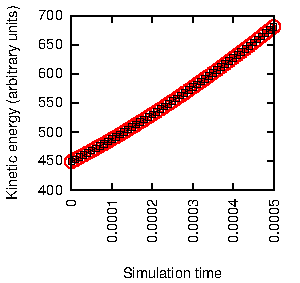
\includegraphics[width=0.4\textwidth]{figs/CodensityTestEk}
\small
\begin{tabular}[b]{l|l|l}
 step & Effective & Simulated \\ \hline
  0 & 0.448474977D+03& 0.448474977D+03\\
 50 & 0.467204101D+03& 0.467204101D+03\\
100 & 0.487015790D+03& 0.487015790D+03\\
150 & 0.507871571D+03& 0.507871571D+03\\
200 & 0.529741404D+03& 0.529741404D+03\\
250 & 0.552597964D+03& 0.552597964D+03\\
300 & 0.576415084D+03& 0.576415084D+03\\
350 & 0.601167084D+03& 0.601167084D+03\\
400 & 0.626828411D+03& 0.626828411D+03\\
450 & 0.653373446D+03& 0.653373446D+03\\
500 & 0.680776383D+03& 0.680776383D+03
\end{tabular}
 \caption{Evolution of the kinetic energy in the simulated and effective
 codensity formulations. No differences can be found.}
 \label{f:testDD}
\end{figure}

\section{Boundary conditions}
\label{s:boundaryConditions}
Boundary conditions are imposed for each quantity being evolved through
equations~\ref{e:NavierStokes}-\ref{e:induction} and \ref{e:composition}.
For the temperature and composition, the boundary conditions are applied to the
quantity being evolved plus the underlying static radial profile. The possible
boundary conditions and the option values for the config file (see
section~\ref{s:runConfig}) are shown in the following sections.

\subsection{Boundary conditions on the flow}
Besides obeying a non penetration condition, at each boundary the velocity
field obeys one of the following conditions:
\begin{itemize}
\item Free slip (0). Sets the radial gradient of the flow to 0 at the boundary.
\item No slip (1). Sets the flow to 0 at the boundary.
\end{itemize}

\subsection{Boundary conditions on the temperature}
At each boundary, the temperature obeys one of the following conditions:
\begin{itemize}
 \item Fixed/constant temperature (0).
       This fixes the temperature anomalies to be 0 at the boundary.
       It also fixes the static temperature profile to be a conductive profile.
 \item Fixed/constant heat flux (1).
       Fixes the radial gradient of the temperature anomalies to be 0 at
       the boundaries. It also fixes the static temperature profile to be
       nearly adiabatic.
\end{itemize}

\subsection{Boundary conditions on the magnetic field}
At each of the boundaries, the magnetic field obeys one of the following
conditions:
\begin{itemize}
 \item Vacuum (0);
 \item Pseudo-vacuum (1);
\end{itemize}

\subsection{Boundary conditions on the composition}
At each boundary, the composition obeys one of the following conditions:
\begin{enumerate}
 \item Fixed/constant composition (0);
 \item Fixed/constant chemical flux (1).
\end{enumerate}


\chapter{Discretization and numerical methods}

\section{Poloidal/toroidal decomposition}
Being solenoidal vector fields, that is, divergence free vector fields, $\vec u$
and $\vec B$ can be represented uniquely in terms of poloidal and toroidal
components,
\begin{subequations}
\begin{gather}
\vec u = \nabla \times ( \nabla \times (v \vec r) +
         r \nabla \times ( w \vec r) \enspace , \\
\vec B = \nabla \times ( \nabla \times (h \vec r) ) +
         \nabla \times ( g \vec r) \enspace .
\end{gather}
\end{subequations}
Notice that the decomposition is different for the flow and the magnetic field.
This difference in decomposition justifies the difference in implementation of
the laplacians, spectral-to-real and real-to-spectral transformations in the
radial direction. The difference in implementation of the flow decomposition has
its justification in that values of the flow coefficients under this expansion
are better numerically behaved \citep{Tilgner1999}.

The scalar fields $v$, $w$, $g$\ and $h$ can then be decomposed in terms of
orthogonal polynomials.

\section{Polynomial decompositions}
One of the main reasons behind the being of spectral codes is that, by expanding
all the scalar field in a basis of orthogonal polynomials, one can transform the
set of coupled partial differential equations into a set of coupled algebraic
equations that can then be solved by standard matrix decomposition/inversion
techniques. Furthermore, differentiation becomes an exact procedure under this
framework, thus reducing numerical errors.

There are, however, downsides to this approach. Some of the gains in speed and
accuracy achieved by using a spectral method are, for very high resolutions,
overcome by the need to perform all multiplications in real space and,
therefore, all the forward/backward transform overhead. This has obvious
consequences for parallelization. Furthermore, care must be taken when
truncating the series of polynomials; the non-linear terms in the equations
involved couple the large and modelled scales to the small (sub-grid,
un-modelled) scales in a non-trivial manner. This is a normally overlooked
problem but a rule of thumb is that for all the cross-scale interactions to be
negligible, all of the spectra of all the quantities being evolved should decay
by at least three orders of magnitude between the highest and the lowest power.

DRS uses a spectral decomposition in both horizontal and radial direction.
Chebyshev polynomials are used in the radial direction and Spherical Harmonics
are used in the horizontal. The next subsections are dedicated at the details
of these expansions.

\subsection{Spherical harmonic decomposition}
\label{s:SphericalHarmonicDecomp}

We use $4\pi$ normalised spherical harmonics, defined as :
\begin{equation}
 Y_\ell^m( \theta , \varphi ) =  \sqrt{(2\ell+1)\frac{(\ell-m)!}{(\ell+m)!}} \, P_\ell^m ( \cos{\theta} )\, e^{i m \varphi },
\end{equation}
where $P_\ell^m ( \cos{\theta} )$ are the un-normalized Associated Legendre
Polynomials (ALP) and
\begin{equation}
 \int Y_\ell^m( \theta , \varphi ) {Y^*}_\ell^m( \theta , \varphi ) \mbox{d}\Omega = 4\pi.
\end{equation}

The polynomials
$\bar{P}_\ell^m ( \cos{\theta} ) = \sqrt{(2\ell+1) \frac{(\ell-m)!}{(\ell+m)!}}$
are the normalised ALP, which we use throughout the code to construct the
spherical harmonics.

\warning{Before version 1.6.0 (MAGIC numbers 101**) we used un-normalised ALP.
After and including DRS 1.6.0 we use the new $\bar{P}_\ell^m ( \cos{\theta} )$.
This reflects on the imported and exported coefficients. The new code, however,
is smart enough to recognise this situation and read coefficients with any of
these normalisations. Other codes may not!!!}

A scalar function $f(\theta, \varphi)$ can, therefore, be written as:
\begin{equation}
 f(\theta, \varphi) = \sum_{l=0}^L\sum_{m=-l}^{l} Y_\ell^m( \theta , \varphi ) f_l^m.
\end{equation}

\subsubsection{Recurrence relations for the Associated Legendre Polynomials}
\begin{align}
 (\ell-m+1)P_{\ell+1}^{m}(x) &= (2\ell+1)xP_{\ell}^{m}(x) - (\ell+m)P_{\ell-1}^{m}(x)\\
 (1-x^2)\frac{d}{dx}{P_\ell^m}(x) &= \frac1{2\ell+1}
  \left[ (\ell+1)(\ell+m)P_{\ell-1}^m(x) \right. \nonumber \\
   &\quad \left. - \ell(\ell-m+1)P_{\ell+1}^m(x) \right]
\end{align}

\subsection{Chebyshev decomposition}
\label{s:ChebyshevDecomp}
Chebyshev polynomials of the first kind, $y=T_n(x)$, are the real valued
functions solving the Chebyshev partial differential equation:
\begin{equation}
 (1-x^2)\frac{\partial^2 y}{{\partial x}^2} - x\frac{\partial y}{\partial x} +
  n^2 y = 0,
\end{equation}
where $n$ is an integer number greater than or equal to zero.
They can easily be generated by a recurrence relation as follows:
\begin{subequations}
\begin{align}
 T_0(x) &= 1 \label{e:ChebyshevRecur1} \\
 T_1(x) &= x \label{e:ChebyshevRecur2} \\
 T_n(x) &= 2xT_n(x) - T_{n-1}(x) \label{e:ChebyshevRecur3}
\end{align}
\end{subequations}

Alternatively they can be defined as the unique polynomials satisfying:
\begin{equation}
 T_n(\cos(\theta)) = \cos(n\theta), %\label{e:ChebyshevTrig}
\end{equation}
where $\theta$ is any angle in the domain $[0:2\pi[$ and not the colatitude.
From this alternative definition we gather that the Chebyshev polynomials vary
in the interval $[-1,1]$.

In the present code, decompositions in the radial direction are made using
Chebyshev polynomials.

First, we decompose the radial domain into a series of $N_r$ adimensional radial
nodes $r_n$ (see section~\ref{s:problemSetup} for the problem setup). Recall
that in adimensional terms, the shell thickness has size 1 and the radial
coordinate starts at $r_i = \eta/(1-\eta)$, $\eta$ being the aspect ratio of the
shell:
\begin{equation}
r_k = r_i + \frac{1}{2} \left[x_k+1\right],
\end{equation}
with $x_k=\cos\left( \frac{\pi(k-1)}{Nr-1} \right)$. The Chebyshev coordinate
can be written in terms of the radial coordinate as:
\begin{equation}
x_k = 2(r_k-r_i)-1
\end{equation}

Notice that this is a mapping between $x_k=\cos(\theta_k)$ and $r_k$.
Figure~\ref{f:radialNodes} shows a schematic diagram of the positions of the
radial nodes for the case of 31 points and an aspect ratio $\eta=0.35$.
\begin{figure}[htb]
\centering 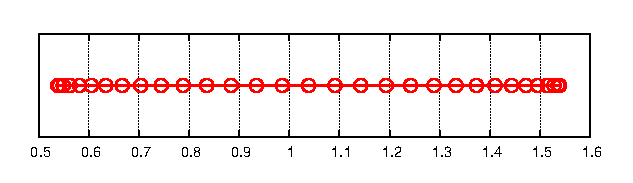
\includegraphics[width=0.9\textwidth]{figs/radialPoints}
 \caption{Positions of the radial nodes for the case of 31 points and an aspect
ratio $\eta=0.35$}
 \label{f:radialNodes}
\end{figure}

A function $f$ depending on the radial coordinate $r$ can then be written as:
\begin{equation}
 f(r) = \sum_n^N f_n T_n(x(r))
\end{equation}

\subsubsection{Normalization}
\begin{equation}
 \int_{-1}^{1} \mbox{d}x T_n(x)\frac{1}{\sqrt{1-x^2}}T_m(x) =
 \left\{
\begin{array}{lcl}
 0 &:& n \ne m \\
 \pi &:& n = m = 0\\
 \pi/2 \quad &:& n = m \ne 0\\
\end{array}
\right.
\end{equation}


\subsection{Spectra}
\label{s:spectra_defs}
In spherical geometry, we can define three types of spectrum: a spectrum in
terms of azimuthal wave number $m$, or {\em m-spectrum}, ${\cal R}_m$; a
spectrum in terms of the spherical harmonic degree $l$, or {\em l-spectrum},
${\cal R}_l$; and a spectrum in terms of the Chebyshev order $n$, or
{\em n-spectrum}, ${\cal R}_n$.

\todo{Be consistent when using $\ell$ vs. $l$.}
For a scalar field, $f(r,\theta, \varphi)$, like the temperature, that can be
decomposed in terms of Spherical Harmonics and Chebyshev polynomials as:
\begin{equation}
 f(r,\theta, \varphi) = \sum_{n=1}^{Nr_s} \sum_{m=0}^{Np_s/2} \sum_{l=m}^{Nt_s}
           T_n(r) Y_\ell^m( \theta , \varphi ) f_{n,l}^m,
\end{equation}
the total energy of that field is constructed as the volume integral
of the square of the field:
\begin{align}
 E &= \iiint f(r,\theta, \varphi)^2 d\Omega\\
   &=\iiint \sum_{n1,n2=1}^{Nr_s} \sum_{m1,m2=0}^{Np_s/2} \sum_{l1,l2=m1,m2}^{Nt_s}
           T_{n1}Y_{l1}^{m1} f_{n1,l1}^{m1}T_{n2}Y_{l2}^{m2} f_{n2,l2}^{m2}\\
   &= 4\pi \sum_{n1,n2=1}^{Nr_s}\int_{r_i}^{r_o}T_{n1}T_{n2}  r^2 \mbox{d}r
      \sum_{m=0}^{Np_s/2} \sum_{l=m}^{Nt_s} f_{n1,l}^{m} f_{n2,l}^{m}\\
\end{align}

This energy can be expressed on a per index base and, therefore, three types of
spectra can be constructed. These are defined as:
\begin{align}
{\cal R}_l & = \sum_{n=1}^{Nr_s}\sum_{m=0}^l  \\
{\cal R}_m & = \sum_{n=1}^{Nr_s}\sum_{l=m}^{Nt_s}  \\
{\cal R}_n & = \sum_{m=0}^{Np_s/2}\sum_{l=m}^{Nt_s}
\end{align}

See section~\ref{s:spectra_files} for the details on how these quantities are
stored in files.

\section{Crank-Nicholson/Adams-Bashford integration}

All of the equations we have to solve are of the form:
\begin{equation}
 \dot f = \partial_t f(\vec{r}, t) =
          \epsilon \nabla^2 f(\vec{r}, t) + F(\vec{r}, t).
 \label{e:toBeSolved}
\end{equation}
The partial derivative on the left hand side has two contributions: $\dot f_1$,
coming from the term with the laplacian and $\dot f_2$, coming from the other
terms. We use a Crank-Nicholson integration for $\dot f_1$ and an Adams-Bashford
integration for the remaining terms.

\subsection{Crank-Nicholson integration}
We start with the Crank-Nicholson integration. Let,
\begin{equation}
\dot f_1(\vec{r}, t) = \epsilon \nabla^2 f(\vec{r}, t).
\end{equation}
We can now discretise in time using index $i$ for the time:
\begin{equation}
\frac{f_1(\vec{r}, t_{i+1}) -f_1(\vec{r}, t_{i})}{t_{i+1}-t_i}
= \epsilon \frac{\nabla^2 f(\vec{r}, t_{i+1}) + \nabla^2 f(\vec{r}, t_{i})}{2}.
\end{equation}
Collecting terms at time $t_{i+1}$ o the l.h.s we get:
\begin{equation}
f_1(\vec{r}, t_{i+1}) - \frac{\epsilon h_i}{2} \nabla^2 f(\vec{r}, t_{i+1})
= f_1(\vec{r}, t_{i}) +  \frac{\epsilon h_i}{2} \nabla^2 f(\vec{r}, t_{i})
\label{e:CN}
\end{equation}
where $h_i = t_{i+1}-t_i$.

This part of the formulation is independent of whether the time-step varies or
not.

% Because of the spherical harmonic decomposition of $f$ and $f_1$ we can write:
% \begin{equation}
% \dot f_1(\vec{r}, t) = \epsilon \left(-\frac{l(l+1)}{r^2} f_l^m(r, t) + \frac{1}{r^2}\partial_r(r^2 \partial_r f_l^m(r, t))\right) Y_l^m(\theta,\phi).
% \end{equation}

\subsection{Adams-Bashford integration}
The forcing part of eq.~\ref{e:toBeSolved} reads:
\begin{equation}
\dot f_2(\vec{r}, t) = F(\vec{r}, t).
\label{e:AB1}
\end{equation}

We use a variable time-step Adams-Bashford integration method to solve this equation.
The Adams-Bashford scheme tells us that, because $F$ is the time derivative of $f_2$ at time $t_i$, then:
\begin{equation}
 f_2(\vec{r}, t_{i+1}) = f_2(\vec{r}, t_{i}) + F(\vec{r}, t_i) h^*_1 - F(\vec{r}, t_{i-1}) h^*_2,
 \label{e:AB}
\end{equation}
with
\begin{eqnarray}
 h^*_1 & = & \frac{h_i}{2h_{i+1}}(2h_{i-1}+h_i),\\
 h^*_2 & = & \frac{h_i}{2h_{i+1}} h_i.
\end{eqnarray}

Notice that the weights $h^*_1$ and $h^*_2$ will reduce to $3h/2$ and $h/2$
respectively when the $h_i$ are constant and equal to $h$. Therefore, our
implementation supports both variable and constant time-stepping (see
section~\ref{s:timeStepping}).

\subsection{Putting it all together}
The iterative solution of eq.~\ref{e:toBeSolved} can now be found by adding
eqs.~\ref{e:CN} and \ref{e:AB} to give the final desired form:
\begin{align}
f(\vec{r}, t_{i+1}) - &\frac{\epsilon h_i}{2} \nabla^2 f(\vec{r}, t_{i+1}) =
 \nonumber \\
= & f(\vec{r}, t_{i}) +  \frac{\epsilon h_i}{2} \nabla^2 f(\vec{r}, t_{i}) +
     F(\vec{r}, t_i) h^*_1 - F(\vec{r}, t_{i-1}) h^*_2.
  \label{e:solvable}
\end{align}

We can now decompose eq.~\ref{e:solvable} in Spherical Harmonics ($Y_l^m(\theta,
\phi)$) and Chebyshev polynomials ($R_n(r)$). The equation for the coefficients
$\tilde f(l,m,n,t_{i+1}$ can then be written as:
\begin{align}
{\cal R}\tilde f(l,m,n, t_{i+1})  &= {\cal R}\tilde f(l,m,n, t_{i}) +\nonumber \\
 &+ R_n(r)\tilde F(l,m,n, t_i) h^*_1 - R_n(r)\tilde F(l,m,n, t_{i-1}) h^*_2.
  \label{e:solvable_spec}
\end{align}


\section{Time-stepping}
\label{s:timeStepping}

Time stepping is controlled via the \verb|delta_t| parameter in the
configuration file (section~\ref{s:runConfig}). Positive values indicate the
constant time step to be used; negative values indicate the initial time step to
be used in an adaptative time step scheme; zero selects an adaptative time
stepping scheme with an initial value ten times smaller than the time step
recorded with the initial state.

\subsection{Adaptative time-stepping}
When an adaptative time stepping scheme is selected, a new value of $h_i$ has to
be selected at each step. Each new vale of $h_i$ is chosen based on a set of
conditions based on the state of the system, namely, the values of the flow
everywhere, the resolution, magnetic field and Coriolis forces strength. The
first three of these conditions is that the time-step $h_i$ cannot be bigger
than the CFL numbers proposed by Glatzmeier \citep{Glatzmaier1984}. A fourth
condition states that the time-step should not be bigger than $1/\sqrt{2\tau}$.

\warning{For stability, when using an adaptative time steping, the number of
radial points should be chosen to be close to the number of theta points. The
same applies to the spectral resolutions.}

\chapter{Input/Output}

\section{Inputs}
\label{s:inputs}
\subsection{State files}
\label{s:stateFiles}
A state file is a text file containing the spherical harmonic coefficients of
a scalar field. The flow state files have extension \verb|.pol| and \verb|.tor|
for the poloidal and toroidal coefficients respectively. The temperature and
composition state files have extensions \verb|.temp| and \verb|.thetac|
respectively. The poloidal and toroidal components of the magnetic field are
stored in files with extension \verb|.Bp| and \verb|.Bt| respectively. The
spectral and physical resolution is described by the accompanying \verb|.par|
file (see section~\ref{s:parFiles})

Each of these files contains only one column of numbers grouped in blocks with
size equal to the number of radial points on input. The loop structure for
reading and writing is:
\begin{verbatim}
do j=1, Npi_s
   do l = m0i*(j/2), Nti_s
      do i=1, Nri
\end{verbatim}
where Nri is the number of radial points, \verb|m0i| is the azimuthal symmetry,
\verb|Nti_s| is the maximum spherical harmonic degree, and \verb|Npi_s| is the
maximum number of real and imaginary coefficients for any degree. l plays the
role of SH degree, \verb|j| plays the role of SH order and \verb|i| is the
radial index starting from the outer boundary.

\subsection{par files}
\label{s:parFiles}
\verb|.par| files describe the state files. They contain, not only the
resolution at which the state files were written, but also the parameter set that
should be used to interpret them. They also contain the simulation time, time
step and sampling rate corresponding to the state files, as well as the
boundary conditions that were applied when creating the state files and the
number of steps since last snapshot. As importantly, they contain the MAGIC
parameters that determines which version of the code they were created with and
is able to appropriately read them. A typical \verb|.par| file looks like:
{\small
\begin{verbatim}
| magic | lformat | lcalc | lheat | lvel | lmag |
  10104       1       4       0       1     0
|  eta   | Prandtl |   Taylor   |  Rayleigh   |  magPr  |
0.350E+00 0.100E+01 0.4000000E+07 0.1000000E+06 0.500E+01
|  Nr  |  Nt  |  Np  |  Nr_s  |  Nt_s  |  Np_s  | lsymm |  m0  |
   33     64     128     33       42       84       0       1
| delta_t | nsteps | transient | sampling_rate | step | time | drift |
 0.500E-04   10000       0           100         000   0.0E+0  0.0E+0
'A useful comment.
\end{verbatim}
}

At this point several formats are available, described by the \verb|magic|
number. Templates for several \verb|magic| numbers are provided in the
templates folder.

The first two lines indicate the base-name for the input and output statefiles
and \verb|.par| files. Next we can find the noise level each variable is to be
initialised to in case the corresponding state file is not found.

The next two lines are particularly worthy of note. They determine the output
format, computation to carry and the boundary conditions to be used for each
quantity. The meaning of each of \verb|temBC|, \verb|compBC|, \verb|flowBC| and
\verb|magBC| is explained in section~\ref{s:boundaryConditions}.

Possible valued for the format, \verb|lformat| are 0 for clear text, unformatted;
any other value for binary formatted output.

\section{Outputs}
\label{outputs}
DRS outputs to several files. At the end of each run, the states of the flow,
field and temperature are dumped to file. The spectra is also saved at this
point.

During the run, DRS saves a number of quantities at the frequency specified by
\verb|sampling_rate|.

\subsection{Quantities saved at the end of the run}
\subsubsection{Spectra}
\label{s:spectra_files}
Spectra are saved at the end of each run. We save two spectra in terms of
spherical harmonic degree (extension \verb|.lspec|) and order (extension
\verb|.mspec|)and a third spectrum in terms of Chebyshev polynomial order
(extension \verb|.nspec|).
Each file contains columns representing the spectra of the flow, temperature, composition and
field if it varies with time.
\begin{itemize}
 \item{\bf c1} degree/order;
 \item{\bf c2} temperature;
 \item{\bf c3} composition (will only be present for compositional runs);
 \item{\bf c4} flow;
 \item{\bf c5} field (optional).
\end{itemize}
See section~\ref{s:spectra_defs} for the definitions of each of these
quantities.

\subsubsection{Time averaged kinetic energies per component}
These quantities are store in a file with extension \verb|.uaz|.
\begin{itemize}
 \item{\bf c1} adimensional radius;
 \item{\bf c2} time averaged mean meridional squared flow;
 \item{\bf c3} instantaneous mean meridional squared flow;
 \item{\bf c4} time averaged mean azimuthal squared flow;
 \item{\bf c5} instantaneous mean azimuthal squared flow.
\end{itemize}

\subsubsection{Radial flow energy}
These files have the extension \verb|.ur|.
\begin{itemize}
 \item{\bf c1} adimensional radius;
 \item{\bf c2} time averaged surface integrated squared radial flow;
\end{itemize}

\subsubsection{Temperature}
These files have the extension \verb|.t|.
\begin{itemize}
 \item{\bf c1} adimensional radius;
 \item{\bf c2} time averaged integrated squared temperature anomaly;
 \item{\bf c3} time averaged integrated temperature anomaly.
\end{itemize}

\subsubsection{Advection}
Stores the advective terms and contributions on average over time as a function
of the radial coordinate. Resulting files have the extension \verb|adv|.

The time average, horizontally integrated advective heat flux is defined as:
\begin{equation}
Q_a(r) = \iint u_r(r,\theta,\phi)(\Theta(r,\theta,\phi)+T_S(r)) \sin\theta
d\theta d\phi,
\end{equation}
where angle brackets ($<>$) represent an  average over the period, $\Delta t$,
covered by the present run.

The heat transferred by diffusion is:
\begin{equation}
Q_d(r) = \iint \partial_r (\Theta(r,\theta,\phi)+T_S(r)) \sin\theta
d\theta d\phi.
\end{equation}

The total heat flux is defined as:
\begin{equation}
Q(r) = r\frac{\partial_r \Theta(r) - Pt Q_d(r)}{-\eta/(1-\eta)^2} + 1.
\end{equation}

.\verb|adv| files have the following structure:
\begin{itemize}
 \item{\bf c1} radius;
 \item{\bf c2} $<Q_a(r)>$, the advective part of convection, horizontally and
time averaged;
 \item{\bf c3} $<Q_d(r)>$, the diffusive part of convection, horizontally and
time averaged;
 \item{\bf c4} $<Q(r)>$, the total time averaged heat flux.
\end{itemize}

\subsection{Frequently probed quantities}
\subsubsection{Energies}
Files with extensions \verb|.eb| and \verb|.ek| store the magnetic and kinetic
energies and are appended to every \verb|sampling_rate| steps.
\paragraph{The magnetic energy} (\verb|.eb|) files have 10 columns with the
following structure in spherical coordinates.
\begin{itemize}
 \item{\bf c1} time
 \item{\bf c2} total magnetic energy
 \item{\bf c3} zonal poloidal equatorially anti-symmetric
 \item{\bf c4} zonal toroidal equatorially symmetric
 \item{\bf c5} non-zonal poloidal equatorially anti-symmetric
 \item{\bf c6} non-zonal toroidal equatorially symmetric
 \item{\bf c7} zonal poloidal equatorially symmetric
 \item{\bf c8} zonal toroidal equatorially anti-symmetric
 \item{\bf c9} non-zonal poloidal equatorially symmetric
 \item{\bf c10} non-zonal toroidal equatorially anti-symmetric
\end{itemize}
Columns 3 to 6 start with the dipole's energy. Columns 7 to 10 starts with the
quadrupole.

\paragraph{The kinetic energy} files have 12 columns  with the following
structure in spherical coordinates.
\begin{itemize}
 \item{\bf c1} time
 \item{\bf c2} total kinetic energy
 \item{\bf c3} zonal poloidal equatorially symmetric
 \item{\bf c4} zonal toroidal equatorially symmetric
 \item{\bf c5} non-zonal poloidal equatorially symmetric
 \item{\bf c6} non-zonal toroidal equatorially symmetric
 \item{\bf c7} zonal poloidal equatorially anti-symmetric
 \item{\bf c8} zonal toroidal equatorially anti-symmetric
 \item{\bf c9} non-zonal poloidal equatorially anti-symmetric
 \item{\bf c10} non-zonal toroidal equatorially anti-symmetric
 \item{\bf c11} helicity in the northern hemisphere
 \item{\bf c12} helicity in the southern hemisphere
\end{itemize}

\subsubsection{Coefficients}
Files storing probed coefficients have extension \verb|.koeu| for the flow and
\verb|koeb| for the magnetic field. These coefficients are stored at every
\verb|sampling\_rate| steps, not just at the end.

\paragraph{Flow coefficients} are stored in files with extension \verb|.koeu|.
Coefficients are taken to be at half radius. Azimuthal symmetry is taken into
account via $m0$ which represents the common factor of all azimuthal wave
numbers. Most cases will have $m0=1$.
\verb|.koeu| files have the following structure:
\begin{itemize}
 \item{\bf c1} time;
 \item{\bf c2} $\Re(tor)$, l=1,m=0, solid body rotation;
 \item{\bf c3} $\Re(pol)$, l=m0, m=m0, Real part of the sectoral poloidal flow
of degree $m0$;
 \item{\bf c4} $\Im(pol)$, l=m0, m=m0, Imaginary part of the sectoral poloidal
flow of degree $m0$;
 \item{\bf c5} $\Re(pol)$, l=2*m0, m=2*m0;
 \item{\bf c6} $\Re(tor)$, l=2*m0+1, m=2*m0.
\end{itemize}

\paragraph{Magnetic field coefficients} are stored in files with extension
\verb|.koeb|. Coefficients are taken to be at half radius. Azimuthal symmetry
is taken into account via $m0$ which represents the common factor of all
azimuthal wave numbers. Most cases will have $m0=1$.
\verb|.koeu| files have the following structure:
\begin{itemize}
 \item{\bf c1} time
 \item{\bf c2} $\Re(tor)$, l=1, m=0, toroidal dipole;
 \item{\bf c3} $\Re(pol)$, l=m0, m=m0, Real part of the sectoral poloidal
field of degree $m0$;
 \item{\bf c4} $\Im(pol)$, l=m0, m=m0, Imaginary part of the sectoral
poloidal field of degree $m0$;
 \item{\bf c5} $\Im(pol)$, l=m0+1, m=m0, Imaginary part of the last tesseral
poloidal field of degree $m0$;
 \item{\bf c6} $\Re(pol)$, l=2*m0, m=2*m0;
 \item{\bf c7} $\Re(pol)$, l=2*m0+1, m=2*m0;
 \item{\bf c8} $\Re(tor)$, l=m0, m=m0;
 \item{\bf c9} $\Re(tor)$, l=m0+1, m=m0;
 \item{\bf c10} $\Re(pol)$ l=1, m=0 poloidal axial dipole.
 \item{\bf c11} $\Re(pol)$ l=2, m=0 poloidal axial quadropole.
\end{itemize}

\subsubsection{CFL numbers}
These files have the extension \verb|.cfl|.
\begin{itemize}
 \item{\bf c1} time;
 \item{\bf c2} based on radial flow;
 \item{\bf c3} based on horizontal flow;
 \item{\bf c4} based on the Coriolis force.
\end{itemize}

\subsubsection{Nusselt number}
The Nusselt number is here defined as
\begin{equation}
 Nu = \frac{\partial_r (T + \Theta)}{\partial_r T }
\end{equation}
and is probed both at the CMB and the ICB.
It is stored in files with the extension \verb|.nu| with the following
structure:
\begin{itemize}
 \item{\bf c1} time;
 \item{\bf c2} Value at the ICB;
 \item{\bf c3} Value at the CMB.
\end{itemize}

\subsubsection{Angular momentum}
The angular momentum is computed as:
\begin{align}
 L_x &= \int -r*(u_\phi\cos\phi\cos\theta + u_\theta\sin\phi)\mbox{d}V \\
 L_y &= \int  r*(u_\theta\cos\phi - u_\phi\sin\phi\cos\theta)\mbox{d}V  \\
 L_z &= \int  r*u_\phi\sin\theta\mbox{d}V
\end{align}
Files storing the angular momentum have extension \verb|.am| and have the following
structure:
\begin{itemize}
 \item{\bf c1} time;
 \item{\bf c2} $L_x$;
 \item{\bf c3} $L_y$;
 \item{\bf c4} $L_z$.
\end{itemize}

\subsubsection{Other files}
\begin{itemize}
\item \verb|.dissB|
\item \verb|.dissu|
\item \verb|.u\_mid|
\item \verb|.uzon|
\end{itemize}

\appendix

\chapter{Utilities}
\section{drs-setup}
\label{util:drs-setup}
\verb|drs-setup| is a tool to generate configuration files for the dynamo
program. It asks you for values for the whole required set of parameters and
provides options. It writes to a file called \verb|drs.conf| if it does not
exist or asks for an alternative name/overwrite if it does.

\section{drs-spectra}
\label{util:drs-spectra}
\verb|drs-setup| is a tool to generate the spectra files described in
section~\ref{s:spectra_files} from state files. It should be invoked as:
\begin{verbatim}
$ drs-spectra <state-name>
\end{verbatim}
where \verb|<state-name>| is the basename of the respective \verb|.par| file
without the extension.

\section{drs2dx}
\verb|drs2dx| is a tool to output the specified quantities in a format that
opendx can understand. \verb|drs2dx| reads an input file called drs.dx.in
with the following format:
\begin{verbatim}
# Basename of the input file.
# It will also be used as the basename of the output files.
io_calc_file_in = e035p34h92

comment = 'A nice comment.'

## Resolution for the render
# Radial
Nr = 33

# Meridional
Nt = 64

# Azimuthal
Np = 129

# Makes a decision about what to render.\n
# Numbers are coded as:\n
#
# a b c d e
# | | | | |>e - component 1, 2 or 3 for vectors, irrelevant for scalars
# | | | |> d - coordinate system or stream lines
# | | |> c - quantity to be ploted
# | |> b - curl, gradient or divergence or 0
# |> a - scalar product with selection or 0
#
#
#  e = 1, 2 or 3 for first second or third coordinate or meridional, azimuthal and poloidal streamlines
#      1 or 2 for total or anomaly scalar fiels
#  d = 1, 2 or 3 for cartesian (x,y,x), spherical (r,t,p) or cyllindrical (s, p, z) components respectively, 4 for streamlines, 0 for none
#  c = 1 for the flow
#      2 for the magetic field
#      3 for the temperature field
#      4 for the composition field
#      5 for the magetic field outside the core (up to ro+1)
#  b = 1 for the curl
#      2 for the gradient
#      3 for the divergence
#      0 for nothing
#  a = 1 for scalar product with flow
#      2 for scalar product with field
#      0 for nothing
#
# For example, if I want the meridional component of the curl of the flow,
# a=0, b=1, c=1, d=2, e=2 so \a what = 01122
what = 1

# The type of rendering to do.
# 1 for volume render
# 2 for meridional cut
render_type = 1

# For cuts, it tells drs2dx where the data is to be taken.
# For volume renders it is unused.
where = 0.0d0
\end{verbatim}

\section{drs-state-change}
Modifies the state on input.
It takes two parameters on the command line: the first is the base name for the
state; the second is an integer indicating which transformation to perform.
At this point the only transformation encoded is the removal of the toroidal
zonal flow, indicated by the value ``0''.

\section{drs-state-average}
Averages a set of states. It reads a configuration file \verb|state-average.in|
of the form:
\begin{verbatim}
# Add the names of states here, one per line.
# First state defines the spatial resolution of the average.
# Any line starting with '#' or '*' is disregarded.
# An example follows:
e035p1t2r100000m1p5test.1
e035p1t2r100000m1p5test.2
\end{verbatim}
Each line corresponds to a state. At present we perform only simple averages of
the states. in the future we want to include proper time averaging.

\section{Utility scripts}
\subsection{compressdata/uncompressdata}
These are probably the most used scripts at the moment. They compress and
uncompress the files of the state using \verb|gzip|.
\subsection{drs\_plot.sh}

\subsection{drs\_cleanRun.sh}
Removes files with extension adv am cfl dissu ek koeu lspec mspec nspec nu t uaz u\_mid ur uzon
\subsection{latestNormalizedSpectra.sh}
Computes and saves the latest normalized spectra of the flow, temperature and composition.
\subsection{resubmitJob.sh}
Resubmits a job to either a pbs queue or a shell
\subsection{rebuildTimeSeries.sh}
Concatenates the files for the energy, etc. for each run into files for the whole set.
\subsection{drs\_plot.sh}
Simplifies plotting equatorial slices of the given quantities.
\subsection{stopRun.sh}
Cleanly stops a run and removes the jobs from any queue they may be in.


\chapter{Benchmarks}
\section{Christensen 2001}
\label{bench:Christ01}
\citet{ChristensenEtAl01} propose a series of quasi-static solutions to the
convective and dynamo problems. For a series of cases they provide global and
pointwise values with confidence intervals any numerical code must reproduce.
In particular, their case 1.a represents a dynamo solution. This solution has
the structure presented in figure~\ref{f:BenchChrist01}.
\begin{figure}[htb]
\centering
 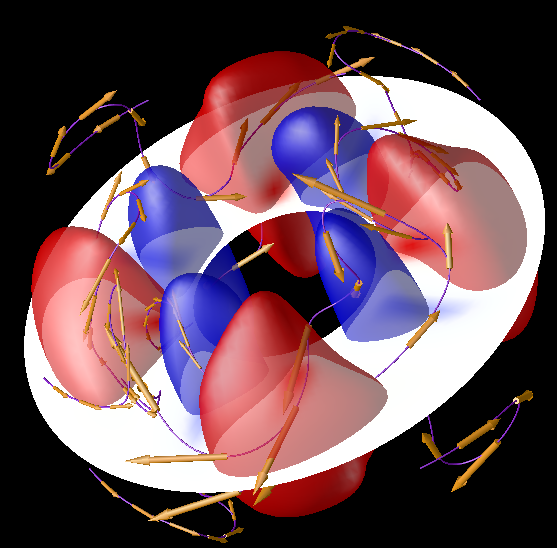
\includegraphics[width=0.45\textwidth]{figs/BenchmarkStructure}
 \caption{Structure of the benchmark solution for case 1.a of
\citep{ChristensenEtAl01}. The dominant flow mode is of SH order 4, as is the
patern of temperature. The whole structure rotates about the system's rotation
axis. In the equatorial plane we ploted the radial component of the flow.
Isosurfaces of temperature are in red for values above the static profile and
in blue for values below. Instantaneous particle trajectories are shown in
purple with velocities overlaied (yellow arrows). The magnetic field is not
represented here.}
 \label{f:BenchChrist01}
\end{figure}

%  Dimensions:    Nr,    Nt,    Np,  Nr\_s,  Nt\_s,  Np\_s
%   Old:          33     64    129     33     64    129

%  Resolution
%    51.853755756495886


\begin{table}
\centering
\begin{tabularx}{0.7\textwidth}{l|rcl|r}
   & \multicolumn{3}{c|}{Reference Values } & Our values \\\hline
Ek &  30.7330 &$\pm$& 0.020   & 30.7199\\
Eb & 626.4100 &$\pm$& 0.40    & 625.6904\\
T  &   0.3734 &$\pm$& 0.00040 &  0.3727\\
up &  −7.6250 &$\pm$& 0.0060  & -7.6826\\
Bt &  −4.9289 &$\pm$& 0.0060  & -4.8958
\end{tabularx}
\caption{Comparison of the results for a run of our code for the benchmark case
1.a of \citep{ChristensenEtAl01}.}
\end{table}


\section{2013/2014}

\bibliography{userManual}
\bibliographystyle{abbrvnat}

\end{document}
